\chapter{Анализ секретности системы квантовой коммуникации с недоверенным приемным узлом} \label{ch:ch6}
\section{Исследование возможностей злоумышленника по получению информации о квантовом состоянии при разделении многофотонных состояний} \label{sec:ch6/sec1}

Let us consider weak coherent state $|\alpha e^{i \varphi}\rangle$, where $\alpha$ is the amplitude of the states and  $\varphi$ is the phase, which encoded the bit. Probability of obtaining an anticipated measurement result indicating the presence of $n$ photons in a given sample or pulse can be obtained by considering the trace of the product of the density matrix of the coherent state $\rho$ and the projector on the Fock basis $|n\rangle\langle n|$: 
%
\begin{align}
    P_n&=\text{Tr}(\rho |n\rangle\langle n|) = \text{Tr}(|\alpha e^{i \varphi}\rangle \langle\alpha e^{i \varphi} |n\rangle\langle n|) \nonumber \\
    &= \text{Tr}(\sum_{k=0}^{\infty}\sum_{m=0}^{\infty} e^{-|\alpha|^2} \frac{(\alpha e^{i \varphi})^k(\alpha^{*} e^{-i \varphi})^m}{\sqrt{k!m!}} |k\rangle\langle m |n\rangle\langle n|) \nonumber  \\
    &=\sum_{j=0}^{\infty}\sum_{k=0}^{\infty}\sum_{m=0}^{\infty} e^{-|\alpha|^2} \frac{(\alpha e^{i \varphi})^k(\alpha^{*} e^{-i \varphi})^m}{\sqrt{k!m!}}\langle j |k\rangle\langle m |n\rangle\langle n|j\rangle \nonumber  \\
    &=e^{-|\alpha|^2} \frac{(|\alpha|^{2n})}{n!}, \label{pnver}
\end{align}
% 
where we used the orthogonality property of Fock basis vectors, $\langle k| n \rangle = \delta_{kn}$, where $\delta_{kn}$ is delta Kronecker symbol. Thus we can present the weak coherent state in Fock Basis as:
%
\begin{equation}
    |\alpha e^{i \varphi}\rangle = e^{-\frac{|\alpha|^2}{2}}\sum_{n=0}^{\infty}  \frac{(\alpha e^{i \varphi})^n}{\sqrt{n!}} |n\rangle.
\end{equation}
%
Therefore, the state after measurement will be reduced as follows:
%
\begin{equation}
    \Tilde{\rho}=\frac{\sqrt{|n\rangle\langle n|} |\alpha e^{i \varphi}\rangle \langle\alpha e^{i \varphi} | \sqrt{|n\rangle\langle n|}}{P_n}.
\end{equation}
%
Lets investigate how operator $\sqrt{|n\rangle\langle n|}$ acts on vectors in the Fock basis $|m\rangle$ presenting it as a taylor series. Lets consider two different cases:
%
\begin{enumerate}
    \item $m \neq n$
    \begin{align}
        \sqrt{|n\rangle\langle n|}|m\rangle = \sum_{k=0}^{\infty} \frac{(-1)^k(2k)!}{(1-2k)(k!)^2 4^k}(|n\rangle\langle n|-\hat{I})^k|m\rangle ,
    \end{align}
    where $\hat{I}$ is identity operator. Using the following properties
    \begin{gather}
        \hat{I}|m\rangle=|m\rangle, \\
        (|n\rangle\langle n|)^k |m\rangle = (|n\rangle\langle n|)^{k-1} |n\rangle\langle n|m\rangle = 0,
    \end{gather}
    we obtain
    \begin{align}
       \sqrt{|n\rangle\langle n|}|m\rangle = \sum_{k=0}^{\infty} \frac{(-1)^k(2k)!}{(1-2k)(k!)^2 4^k}(-1)^k|m\rangle = 0 |m\rangle.
    \end{align}
    \item $m=n$
    
    Then using the next properties
    \begin{align}
        (|n\rangle\langle n|)^k |n\rangle = (|n\rangle\langle n|)^{k-1}=\nonumber\\ =|n\rangle\langle n|n\rangle = (|n\rangle\langle n|)^{k-1} |n\rangle = ... = |n\rangle,
    \end{align}
    then
    \begin{align}
        \sqrt{|n\rangle\langle n|}|n\rangle &= \sum_{k=0}^{\infty} \frac{(-1)^k(2k)!}{(1-2k)(k!)^2 4^k}(|n\rangle\langle n|-\hat{I})^k|n\rangle \nonumber\\
        &=|n\rangle + \sum_{k=1}^{\infty} \frac{(-1)^k(2k)!}{(1-2k)(k!)^2 4^k}(|n\rangle\langle n|-\hat{I})^k|n\rangle \nonumber\\
        &=|n\rangle + 0 = |n\rangle.
    \end{align}
\end{enumerate}
%
Thus the reduced state has the next form:
%
\begin{align}
   \Tilde{\rho}&=\frac{1}{P_n}\sum_{k=0}^{\infty}\sum_{m=0}^{\infty} e^{-|\alpha|^2} \frac{(\alpha e^{i \varphi})^k(\alpha^{*} e^{-i \varphi})^m}{\sqrt{k!m!}} \sqrt{|n\rangle\langle n|}|k\rangle\langle m |\sqrt{|n\rangle\langle n|} \nonumber \\
   &= \frac{1}{P_n} P_n |n\rangle\langle n| = |n\rangle\langle n|. \label{rhored}
\end{align}
%
Thereby according to the equations obtained in eq.~\ref{pnver} and eq.~\ref{rhored} the measurement results  of the number of photons in the pulse (projection on the Fock basis) in weak coherent states and the reduced state after the measurement do not contain information about the phase of the coherent state $\varphi$. In the multimode case, the problem reduces to the single mode case considered above.

\pagebreak

%%%%%%%%%%%%%%%%%%%%%%%%%%%%%%%%%%%%%%%%%%%%%%%%%%%%%%%%%%%%%%%%%%%%%%%%%%%%%%%%%
\section{Характеристики компонентов экспериментального стенда} \label{ch:ch5/sec2}

Значительную трудность представляет согласование спектральных характеристик Алисы и Боба. Даже при использовании одного источника для имитации хорошо скоррелированных лазеров, требуется подобрать оптические фильтры с максимально совпадающими характеристиками. В системе квантовой коммуникации частота модулирующего сигнала равна $\Omega = 4,8$~ГГц (рис.\ref{fig:RF_sin_osc} ). Значит, полоса спектрального фильтра не должна превышать величину $2\Omega$. Для этих целей используются волоконные узкополосные оптические фильтры на основе Брэгговских решеток. На рисунке \ref{fig:Spectrums} показаны измеренные характеристики максимально близких по серединному значению полосы пропускания фильтров. Уровень полуширины (FWHM) первого фильтра ОФ1 равен 48,8~пм (или 6,1~ГГц), а уровень полуширины (FWHM) второго фильтра ОФ2 равен 40~пм (или 5~ГГц). При этом разность центральных длин волн составляет 8~пм (или 1~ГГц). В ходе эксперимента лазер подстраивался таким образом, чтобы минимальная величина засветки от центральной проходила через оба оптических фильтра. Из-за несовпадения их характеристик повышался уровень шумов, вследствие чего ухудшалась видность картины интерференции.  

 \begin{figure}[ht]
  \centering
  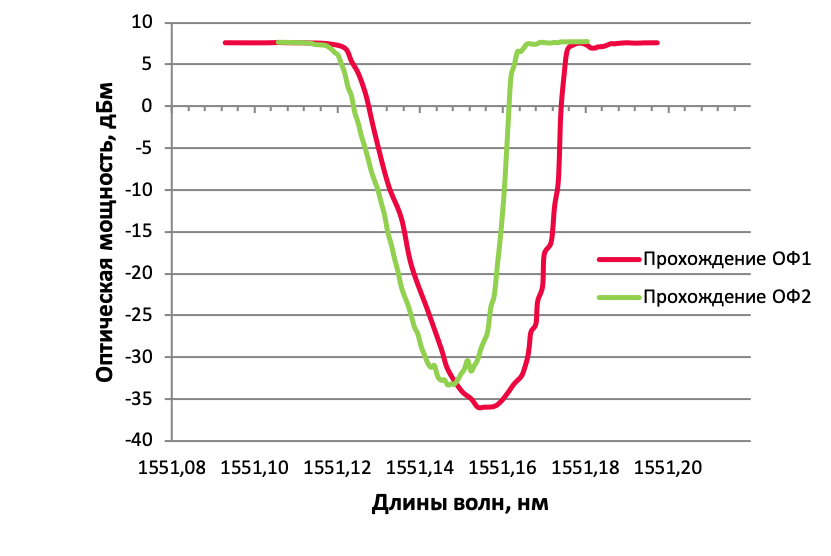
\includegraphics[scale=0.8]{T-spectrums.png}
  \caption{Спектральные характеристики оптических фильтров}
  \label{fig:Spectrums}
\end{figure}

\pagebreak

%%%%%%%%%%%%%%%%%%%%%%%%%%%%%%%%%%%%%%%%%%%%%%%%%%%%%%%%%%%%%%%%%%%%%%%%%%%%%%%%%%%%%%%%%%%%%%%%%%%%%%%%%%%%%%%%%
%\section{Экспериментальный стенд} \label{ch:ch5/sec3}


%\pagebreak

%%%%%%%%%%%%%%%%%%%%%%%%%%%%%%%%%%%%%%%%%%%%%%%%%%%%%%%%%%%%%%%%%%%%%%%%%%%%%%%%%%%%%%%%%%%%%%%%%%%%%%%%%%%%%%%%%
\section{Зависимость интенсивности на боковых частотах от сдвига фаз в результате интерференции в классическом режиме} \label{ch:ch5/sec5}


На первом этапе измерения проводились в классическом режиме с помощью измерителей оптической мощности и нулевом значении вносимых потерь ПОА. При этом один из измерителей мощности $Д3$ служил для обратной связи и подстройки оптической фазы между двумя плечами с помощью $ФМ4$ и $ГЕН2$. Когда разность оптических фаз была скомпенсирована, и центральная мода постоянно наблюдалась в одном из выходных плечей $СД2$, в ручном режиме последовательно производилась смеша фазовых состояний радиочастотных модулирующих сигналов посредством изменения значений в IQ-таблице ЦАПов с шагом $10^{\circ}$. 

В результате наблюдалась картина на рисунке \ref{fig:Experimental_TF_classical}. Значение конструктивной интерференции на первом детекторе составило величину $I_{max}=6,3$~мкВт, а деструктивной -- $I_{min}=0,2$~мкВт, тогда как на втором $I_{max}=6,13$~мкВт, и $I_{min}=0,08$~мкВт, соответственно. 

 \begin{figure}[ht]
  \centering
  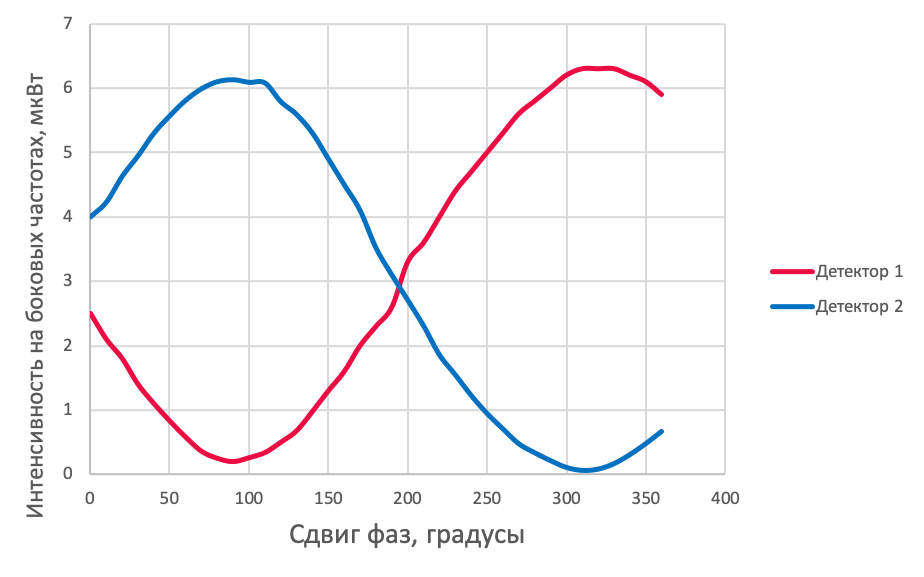
\includegraphics[scale=0.7]{Experimental_TF_classical.png}
  \caption{Зависимость интенсивности на боковых частотах в результате интерференции от разности фаз модулирующих сигналов}
  \label{fig:Experimental_TF_classical}
\end{figure}

Если определить отношение $I_{max}$ к $I_{min}$, как контраст, то в первом плече контраст был равен 31,5, а во втором -- 76.6. Видность интерференционной картины определяется как: 
\begin{equation}
	V=\frac{I_{max}-I_{min}}{I_{max}+I_{min}}
\end{equation}

В первом случае видность составила $V_{1}=93,8\%$, во втором -- $V_{2}=97,4\%$


\pagebreak

%%%%%%%%%%%%%%%%%%%%%%%%%%%%%%%%%%%%%%%%%%%%%%%%%%%%%%%%%%%%%%%%%%%%%%%%%%%%%%%%%%

\section{Вероятности срабатываний детекторов} \label{ch:ch5/sec6}

 Известно, что оптический фильтр отражает центральную оптическую моду ($k=0$). Значит, среднее число фотоном на входе в каждый детектор может быть найдена как \ref{nph1}. 
 
\begin{align}\label{nph1}
    n(\Delta\varphi)_{1,2}&=\mu_0\eta_c\Bigg(\sum_{k\neq 0}|d_{0k}^{S}(\beta)|^2 + \vartheta|d_{0k}^{S}(\beta)|^2 \pm \nonumber \\
    &\pm \cos(\varphi_0)\Big(\sum_{k\neq 0}|d_{0k}^{S}(\beta)|^2e^{i\Delta\varphi k}+ \vartheta|d_{0k}^{S}(\beta)|^2 \Big) \Bigg),
\end{align}

где $\Delta\varphi=\varphi_B-\varphi_A$, $\varphi_0$ это относительная оптическая фаза между импульсами отправителя (Алисы) и получателя (Боб), $\vartheta \ll 1$ часть центральной моды ($k=0$) проходящая через фильтр, ввиду ограниченности его характеристики. Используя свойства d-функци из \cite{varshalovich1988quantum}, можно упростить предыдущее выражение \ref{nph}

\begin{align}
    n(\Delta\varphi)_{1,2}=\mu_0\eta_c\Big(1-(1-\vartheta)(1\mp\cos(\varphi_0))|d_{00}^{S}(\beta)|^2 \pm \nonumber \\
    \pm\cos(\varphi_0)d_{00}^{S}(\beta')\Big) \label{nph},
\end{align}

где аргумент $\beta'$ получен следующим образом \ref{betaappox}. 

\begin{equation} \label{betaappox}
    \cos(\beta')=\cos^2(\beta) \mp \sin^2(\beta)\cos(\Delta\varphi).
\end{equation}

Чтобы оценить вероятность срабатывания воспользуемся линейным приближением Манделя, предполагая слабые интенсивности ($n(\Delta\varphi)_{1,2} \ll 1$):

\begin{eqnarray}
    \mathcal{P}_{1,2}^{+}(\Delta\varphi)=\left(n(\Delta\varphi)_{1,2}\eta_DF+\gamma_{dark}\right)\Delta t, \label{pdet}
\end{eqnarray}

где $\eta_D$ квантовая эффективность, $F$ частота смены состояний, $\gamma_{dark}$ частота темновых отсчетов детектора одиночных фотонов, и $\Delta t$ время окна срабатывания. Для простоты положим $\Delta t F=1$. Отсутствие срабатывания определим, как $\mathcal{P}_{1,2}^{-}(\Delta\varphi)=1-\mathcal{P}_{1,2}^{+}(\Delta\varphi)$.     


Используем несколько полезных приближений, которые помогут оценить квантовый коэффициент ошибок по битам (QBER) и скорости формирования просеянного ключа. Для начала положим, что число взаимодействующих мод велико ($S\rightarrow \infty$), что действительно так для стандартных волоконно-оптических модуляторов. Тогда можно использовать приближение d-функций следующим образом:

\begin{align}
d_{nk}^S(\beta) &\xrightarrow{S\rightarrow \infty} J_{n-k}(m), \label{limdj} \\
\beta &\propto m, \label{propto}
\end{align}
где $J_k(m)$ функция Бесселя первого порядка. Полагая значение $m$ малым, что действительно так, в соотвествии с теорией классической модуляции воспользуемся приближением первого порядка функции Бесселя. 


Так в соответствии с уравнение \ref{betam} $\beta \rightarrow 0$, следовательно можно использовать аппроксимации первого порядка для выражения \ref{betaappox} в терминах $m$ подразумевая пропорциональность в уравнении \ref{propto}.


Определим уравнение~\ref{pdet} следующим образом:

\begin{align}\label{pdet1}
 \mathcal{P}_{1,2}^{+}(\Delta\varphi)&=\mu\eta\Big(1\pm\cos(\Delta\varphi)\cos(\varphi_0)\Big)+ \nonumber
 \\
 &+\vartheta\Big(\mu_c\eta(1\pm\cos(\varphi_0))\Big)+p_{dark},
\end{align}


где $\eta$ полная оптическая пропускная способность квантового канала с учетом квантовой эффективности детектора, $p_{dark}=\gamma_{dark}\Delta t$ это вероятность темнового срабатывания во временном интервале $\Delta t$, и $\mu$ и $\mu_c$ это среднее число фотонов на боковых и на центральной моде соотвественно после модуляции, как определено:

\begin{align}
    \mu&=\mu_0\sum_{k\neq 0}|d_{0k}^{S}(\beta)|^2, \\
    \mu_c&=\mu_0-\mu=\mu_0(1-\sum_{k\neq 0}|d_{0k}^{S}(\beta)|^2).
\end{align}
Выраение в уравнени~\ref{pdet1} даёт точное соотношение между экспериментальными параметрами и показывает, как они влияют на вероятности детектирования квантовых состояний. 


\pagebreak

%%%%%%%%%%%%%%%%%%%%%%%%%%%%%%%%%%%%%%%%%%%%%%%%%%%%%%%%%%%%%%%%%%%%%%%%%%%%%%%%%%
\section{Зависимость интенсивности на боковых частотах от сдвига фаз в результате интерференции в режиме счета фотонов} \label{ch:ch5/sec7}



 \begin{figure}[ht]
  \centering
  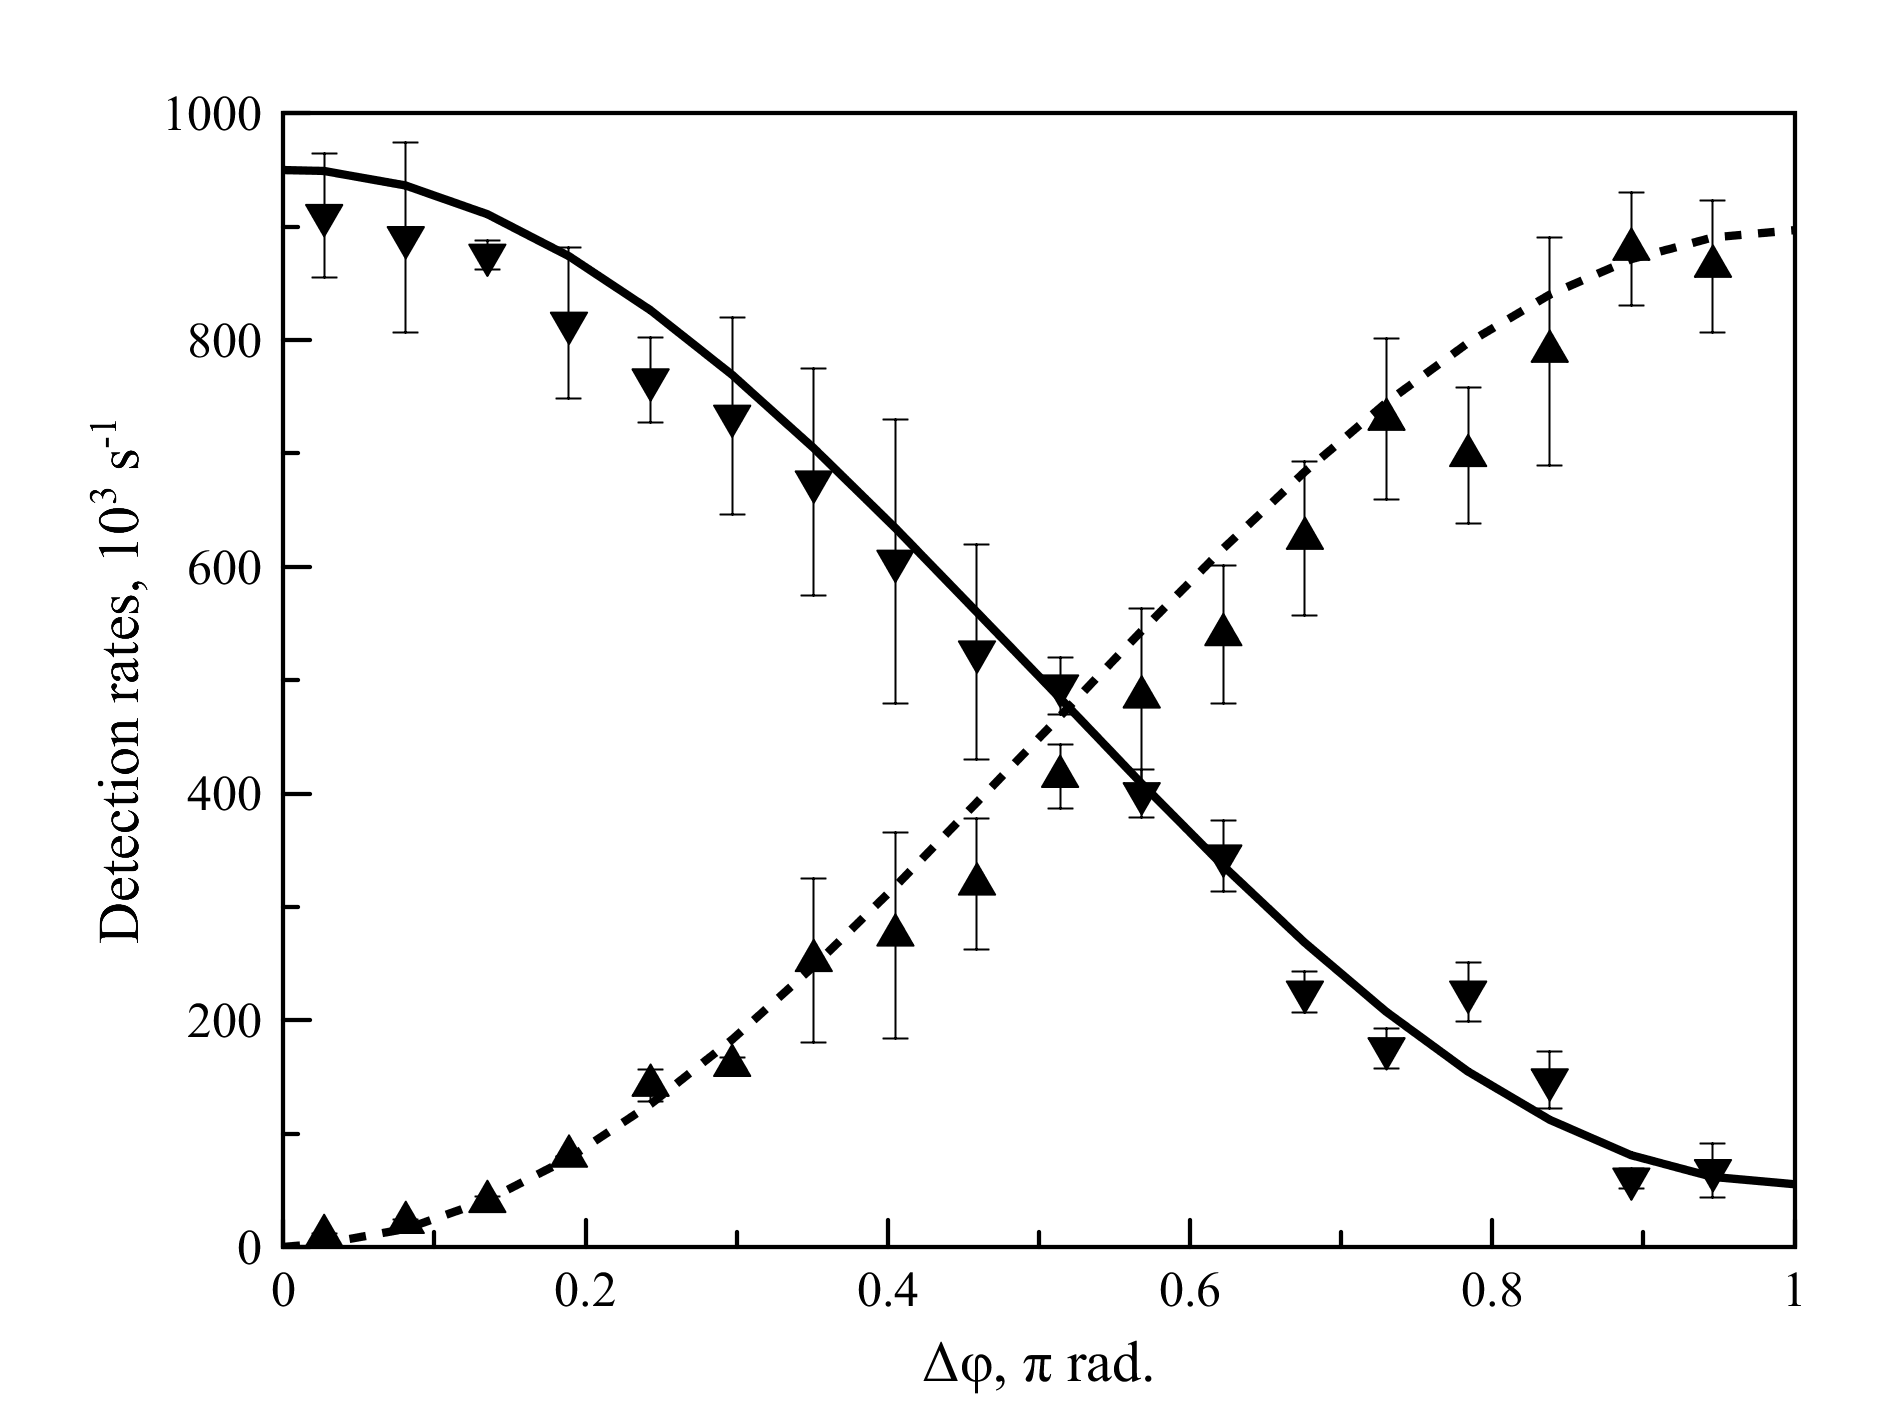
\includegraphics[scale=0.2]{ExperimentTF.png}
  \caption{Зависимость количества отсчетов в результате интерференции от разности фаз модулирующих сигналов}
  \label{fig:Experimental_TF}
\end{figure}


\pagebreak

%%%%%%%%%%%%%%%%%%%%%%%%%%%%%%%%%%%%%%%%%%%%%%%%%%%%%%%%%%%%%%%%%%%%%%%%%%%%%%%%%%
\section{Оценка коэффициента битовых ошибок и скорости формирования ключа} \label{ch:ch5/sect8}

Далее рассмотрим только те случаи, где срабатывание происходит только на одном из детекторов в единицу времени.  Таким образом, вероятности срабатываний $R$ определяются как:

\begin{align}
    R&=\Big(\mathcal{P}_{1}^{+}\mathcal{P}_{2}^{-}(\Delta\varphi=\varphi_m)+\mathcal{P}_{1}^{-}\mathcal{P}_{2}^{+}(\Delta\varphi=\pi+\varphi_m)+ \nonumber \\
    &+\mathcal{P}_{1}^{+}\mathcal{P}_{2}^{-}(\Delta\varphi=\pi+\varphi_m)+\mathcal{P}_{1}^{-}\mathcal{P}_{2}^{+}(\Delta\varphi=\varphi_m)\Big),
\end{align}


где $\varphi_m$ средняя величина несоответствия фаз $\varphi_A$ и $\varphi_B$. Первые два слагаемых - это вероятности успешного определения битов легитимными пользователями, тогда как оставшиеся два слагаемых - вероятности смены бита на противоположный (bitflip) (полагая $\varphi_0 \approx 0$). Таким образом, можно определить выражение для QBER $Q$ следующим образом:

\begin{align}
    Q=\frac{\mathcal{P}_{1}^{-}\mathcal{P}_{2}^{+}(\Delta\varphi=\varphi_m)+\mathcal{P}_{1}^{+}\mathcal{P}_{2}^{-}(\Delta\varphi=\pi+\varphi_m)}{R}.
\end{align}


Наконец, можно определить выражение для оценки среднего значения скорости формирования просеянного ключа $K$ (одинаковые биты между легитимными пользователями, но коррелирующие с возможным результатом у злоумышленника, что требует проведения процедуры усиления секретности)
\begin{equation}
    K=FR(1-h(Q)),
\end{equation}
где $h(Q)$ это функция двоичной энтропии. 

\pagebreak

%%%%%%%%%%%%%%%%%%%%%%%%%%%%%%%%%%%%%%%%%%%%%%%%%%%%%%%%%%%%%%%%%%%%%%%%%%%%%%%%%%
\section{Выводы по главе} \label{ch:ch5/sec9}


В \ref{ch:ch5} главе показано, что в результате интерференции квантового фазомодулированного сигнала на боковых частотах на симметричном светоделителе в схеме квантовой рассылки ключа с узлом регистрации, независящим от легитимного пользователя, происходит спектральное разделение квантового сигнала и сигнала на центральной длине волны с их независимой регистрацией в разных плечах светоделителя. 

\pagebreak

